\documentclass{article}

\usepackage[utf8]{inputenc}
\usepackage[top=2cm, left=2cm, right=2cm, bottom=2cm]{geometry}
\usepackage{graphicx}

\title{Homework 2 - Decision Trees \\
        \vspace{5px} \large UTFPR - CPGEI - Data Mining \\
        Prof. Dr. Heitor Silvério Lopes}
\author{Vinícius Couto Tasso}
\date{October, 2019}

\begin{document}

\maketitle

\section*{Hepatitis dataset}


\indent The hepatitis dataset contains data about a group of 155 people with acute and chronic hepatitis. Of all patients, 122 survived and 33 died. The goal is to predict a patient's chance of survival based on their available data.

In order to do so, decision trees were used. Both the ZeroR and the OneR methods' purpose is to establish a baseline to compare the performance of JRip and J48. Table \ref{tab:training_set} presents the results obtained on the evaluation of all methods used.

It is important to note that the baseline methods have such a high accuracy due to a highly imbalanced dataset. As mentioned before, the class that comprises the patients that survived is almost 4 times bigger than the remaining class.

\begin{table}[htp]
    \begin{tabular}{c|c|c|c|c|c|c}
         & Accuracy & TP-Rate (live) & FP-Rate (live) & TP-Rate (die) & FP-Rate (die) & Tree (size / leaves) \\ \hline
         ZeroR & 0.793 & \textbf{1.000} & 1.000 & 0.000 & \textbf{0.000} & 1 / 1 \\
         OneR & 0.845 & 0.951 & 0.563 &  0.438 & 0.049 & 1 / 2 \\
         JRip & 0.877 & 0.894 & \textbf{0.188} & \textbf{0.813} & 0.106 & 7 / 4  \\
         J48 & \textbf{0.922} & 0.984 & 0.313 & 0.688 & 0.016 & 21 / 11 \\
    \end{tabular}
    \caption{Results of the methods applied to the dataset with validation on training set. All methods used the default parameters of Weka version 3.8.3.}
    \label{tab:training_set}
\end{table}

Both ZeroR and OneR are simple classification rules. ZeroR simply predicts the class of the majority. Since, in this case, the majority class represents almost 80\% of the entire dataset, the accuracy will be consequently high. However, high accuracy rates do not necessarily mean that the model is appropriate for the classification task at hand, especially when dealing with imbalanced datasets.

OneR, on the other hand, is a bit more sophisticated. It will try to predict the class based on a single attribute. The attribute of choice will be the one with the lesser prediction error of all. That means that there will be a different rule for every attribute, and the one that performs the better will be used for classification.

Here something quite interesting can be seen. Even with just one attribute out of twenty, the method can reach an accuracy rate of 84,5\%. Not only that, but the true positives (TP) rate of the \textit{live} class is quite high as well. However, further analysis shows that the false positives (FP) rate of this same class is awfully high. 

This suggests that the attribute selected by OneR, ascites\footnote{The accumulation of fluid in the peritoneal cavity, causing abdominal swelling.}, when indicating the absence of this condition on the patient, is a strong indication that chances of survival are high, but it isn't enough to make, by itself, a more accurate prediction about the patients' chance of not surviving.

Both JRip and J48 achieved good accuracy and TP rates for the \textit{live} class. Even though J48 correctly identified 98,4\% of the instances of \textit{live} class, it came with a cost. In order to achieve such a high success rate for the first class, the tree classified many instances of the second class incorrectly. This can be easily identified by looking at the false positives rate of \textit{live} and true positives of \textit{die}. This can be particularly problematic for a scenario like the one presented, where an incorrect prediction (especially a \textit{live} false positive) can have such a negative impact.

Although JRip is less assertive when it comes to classifying the first class, it performs much better overall in this case. It does a much better job at identifying instances of the class \textit{die}, where J48 would incorrectly predict \textit{live}. Not only that, but the size of the tree and, therefore, its complexity, is much smaller.  That makes the task of understanding the logic behind the decision tree much easier.

The same experiments were repeated with cross-validation, instead of validating the model on the same data used in training. The results can be observed in Table \ref{tab:cross_validation}. The results show that the performance got worse, but that's expected. This is due to the fact that, in the first experiment, the validation happened on data that was already known, i.e. data that was used during training. With cross-validation, the validation data is never the same as the one used when learning the model. This is important to evaluate how the model deals with unknown data.

\begin{table}[htp]
    \begin{tabular}{c|c|c|c|c|c|c}
         & Accuracy & TP-Rate (live) & FP-Rate (live) & TP-Rate (die) & FP-Rate (die) & Tree (size / leaves) \\ \hline
         ZeroR & 0.793 & \textbf{1.000} & 1.000 & 0.000 & \textbf{0.000} & 1 / 1 \\
         OneR & 0.800 & 0.935 & 0.719 &  0.281 & 0.065 & 1 / 2 \\
         JRip & 0.780 & 0.894 & 0.656 & 0.344 & 0.106 & 7 / 4 \\
         J48 & \textbf{0.838} & 0.943 & \textbf{0.563} & \textbf{0.438} & 0.057 & 21 / 11 \\
    \end{tabular}
    \caption{Results of the methods applied to the dataset with cross-validation with 10 folds. All methods used the default parameters of Weka version 3.8.3.}
    \label{tab:cross_validation}
\end{table}

The results show that validating the model with cross-validation favors the J48 approach. Even though this is a more complex method than the JRip, the numbers show that its results far exceed the ones achieved by the other methods. Here we can see that the TP rate of \textit{live} is significantly higher when using cross-validation, compared with validation on the training set. This means that the methods have much more difficulty separating both classes.


\section*{Soybean dataset}

The soybean dataset is composed of 683 instances of soybean affected by 19 different types of diseases. The purpose of this dataset is to determine the diagnostic of a given soybean. 

According to the J48 method, the attribute that provides the greatest separability of classes is \textit{leafspot-size}. The last class, represented by 18 in Figure \ref{fig:confusion_matrix}, had the worst accuracy rate. This is due to the fact that it has the least amount of samples, with only 8 samples to represent it, while the average amount of samples per class on this dataset is roughly 34.

\begin{figure}[htp]
    \centering
    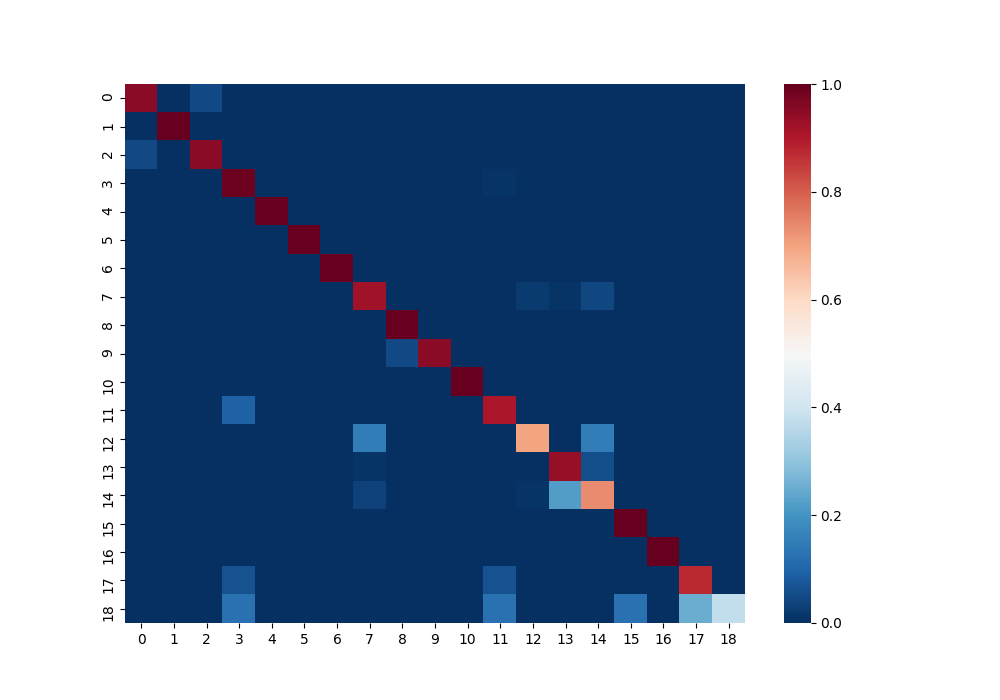
\includegraphics[scale=0.6]{confusion_matrix.png}
    \caption{Confusion matrix using J48 for the original dataset.}
    \label{fig:confusion_matrix}
\end{figure}

Literature suggests removing the four classes with the least amount of samples from the dataset for the classification task. A comparison between both approaches is shown in Table \ref{tab:comparison}. With the modified dataset, the attribute that provides the greatest separability is \textit{int-discolor}. 

\begin{table}[htp]
    \centering
    \begin{tabular}{c|c|c}
         & 19 classes & 15 classes \\ \hline
         Accuracy & 0.915 & 0.915 \\
         AUC &  0.983 & 0.982 \\
         Leaves & 61 & 59 \\
         Tree & 93 & 89 \\
         Worst recall class & herbicide-injury & frog-eye-leaf-spot \\
    \end{tabular}
    \caption{Comparison of classification between the entire dataset, containing 19 classes, and the reduced dataset, with 15 classes.}
    \label{tab:comparison}
\end{table}

On the original dataset, the class with the worst accuracy rate is \textit{herbicide-injury}, the class with the least amount of samples. After cleaning up the dataset, this class is removed and another class takes its position. The reduction on the dataset doesn't seem to affect much the classification process, but it does reduce the tree size, making it less complex, and eliminates what could be considered ``noise'' for the other classes.

As stated before, the \textbf{c} parameter of the J48 method used was the default value of Weka. This parameter is responsible for establishing the minimum amount of instances per leaf. In order to find the optimal value for \textbf{c}, a series of tests were performed by varying its value from 2 to 10, as shown in Table \ref{tab:c_optimal}.

\begin{table}[htp]
    \centering
    \begin{tabular}{c|c|c|c|c}
         \textbf{c} & Accuracy & AUC & Tree size & Leaves \\ \hline
         2 & 0.915 & 0.982 & 89 & 59 \\ 
         3 & 0.907 & 0.984 & 82 & 56 \\
         4 & 0.904 & 0.985 & 69 & 47 \\
         5 & 0.896 & 0.986 & 67 & 45 \\
         6 & 0.893 & 0.984 & 61 & 41 \\
         7 & 0.876 & 0.984 & 50 & 34 \\
         8 & 0.876 & 0.983 & 51 & 35 \\
         9 & 0.869 & 0.983 & 51 & 35 \\
         10 & 0.865 & 0.984 & 47 & 32 \\
    \end{tabular}
    \caption{Comparison of generated trees with different values for the \textbf{c} parameter.}
    \label{tab:c_optimal}
\end{table}

The results show that the best value for AUC is obtained when $\textbf{c} = 5$. Besides the better AUC value, the generated tree is significantly less complex than the original one, generated with $\textbf{c} = 2$. The accuracy loss is very small, only 2\%, which makes the value of 5 ideal for \textbf{c}.

\end{document}
 